% \documentclass{beamer}
\documentclass[xcolor=dvipsnames]{beamer}
\usefonttheme{serif}
%% \usecolortheme[named=Blue]{structure}
\setbeamersize{text margin left=30mm, text margin right=30mm}
\useoutertheme{infolines}
%% \usetheme[height=7mm]{Rochester}
\usetheme{Pittsburgh}
\setbeamertemplate{items}[ball]
\setbeamertemplate{blocks}[rounded][shadow=true]
\setbeamertemplate{navigation symbols}{}

\usepackage[utf8x]{inputenc}
%% \usepackage{default}
\usepackage[english]{babel}
\usepackage{geometry}
%% \usepackage{fullpage}
\usepackage{amsmath, amsthm, amssymb}
\usepackage{listings}
\usepackage{pxfonts}
%% \usepackage{caption}
\usepackage[labelformat=empty]{caption}

%% \usepackage{xcolor}
%% \usepackage{newunicodechar}
%% \newcommand\Warning{%
%%  \makebox[1.4em][c]{%
%%  \makebox[0pt][c]{\raisebox{.1em}{\small!}}%
%%  \makebox[0pt][c]{\color{red}\Large$\bigtriangleup$}}}%
%% \newunicodechar{⚠}{\Warning}

\usepackage{stackengine}
\usepackage{scalerel}
\usepackage{xcolor}
\newcommand\dangersign[1][2ex]{%
  \renewcommand\stacktype{L}%
  \scaleto{\stackon[1.3pt]{\color{red}$\triangle$}{\tiny\bfseries !}}{#1}%
}


%% \usepackage{color}
%% \usepackage{graphicx}
%% \usepackage{natbib}
%% \usepackage{array}
%% \usepackage{booktabs}
%% \usepackage{tabu}
%% \usepackage[utf8]{inputenc}
%% \usepackage{fancyhdr}
%% \usepackage{float}
%% \usepackage{subfigure}
%% \usepackage{titlesec}

\setbeamertemplate{headline}{}
\setbeamertemplate{footline}[frame number]{}
\setbeamertemplate{navigation symbols}{}
\setbeamertemplate{footline}{}
\setbeamertemplate{footline}[frame number]


\def\CCT{{C\nolinebreak[4]\hspace{-.05em}\raisebox{.4ex}{\tiny\bf ++}}}
\def\CC{{C\nolinebreak[4]\hspace{-.05em}\raisebox{.4ex}{\small\bf ++}}}


\definecolor{lstgray}{gray}{0.93}
\definecolor{strgray}{gray}{0.4}

\lstset{ %
  escapechar=@,
  language=C++,
  basicstyle=\footnotesize\ttfamily,
  %% basicstyle=\ttfamily,
  %% keywordstyle=\color{blue}\ttfamily,
  keywordstyle=\bfseries,
  stringstyle=\color{strgray}\ttfamily,
  commentstyle=\color{OliveGreen}\ttfamily,
  %% morecomment=[l][\color{red}]{\#},
  morecomment=[l][\color{blue}]{\#},
  backgroundcolor=\color{lstgray},
  %% keywordstyle=\color{red},
  frame=f,
  frameround=ffff,
  tabsize=2,
  breaklines=true,
  breakatwhitespace=false,
  showspaces=false,
  showstringspaces=false,
  xleftmargin=5pt,
  xrightmargin=5pt,
  morekeywords={in,out,ref,auto,inout,import,ushort,scope,exit,mixin,decltype,varid,sizeof,constexpr,size\_t,string}
}

\def\redcolor{\color{red}}
\def\bluecolor{\color{blue}}
\def\blackcolor{\color{black}}
\def\graycolor{\color{gray}}
\def\greencolor{\color{OliveGreen}}


\def\sectionname{\translate{Section}}
\def\insertsectionnumber{\arabic{section}}
\setbeamertemplate{section page}
{
  \begin{centering}
    \begin{beamercolorbox}[sep=4pt,center]{part title}
      \usebeamerfont{section title}\insertsection\par
    \end{beamercolorbox}
  \end{centering}
}
\def\sectionpage{\usebeamertemplate*{section page}}


\AtBeginSection{\frame{\sectionpage}}


\title{Compile time adjoint in \CC}
\subtitle{22\textsuperscript{nd} EuroAD Workshop, Imperial College}
\author{Dominic Jones}
\date{\small{July 2019}}
\institute{\small{\texttt{github.com/DominicJones}}}


\begin{document}
\begin{frame}[plain]
  \titlepage
\end{frame}


\begin{frame}[fragile]{Overview}
  \begin{enumerate}
  \item {\bf Preliminaries:} resources, basic ideas, etc \vspace{5mm}
  \item {\bf Mapping indices:} separate tree structure and its data \vspace{5mm}
  \item {\bf Language extensions:} functionality that would be very helpful \vspace{5mm}
  \end{enumerate}
\end{frame}


%%
\section{Preliminaries}
%%

\begin{frame}[fragile]{Zero or more}
\begin{lstlisting}
// no state, but instantiable
template<class... T> struct @\aftergroup\bluecolor@list@\aftergroup\blackcolor@ {};
\end{lstlisting}

~

\begin{lstlisting}
// a more useful form...
template<class T, T...> struct @\aftergroup\bluecolor@seq@\aftergroup\blackcolor@ {};
\end{lstlisting}

~

\begin{lstlisting}
// _the_ operation
template<class L> struct front;

template<template<class...> class L, class @\aftergroup\bluecolor@T1@\aftergroup\blackcolor@, class... T>
struct front<L<@\aftergroup\bluecolor@T1@\aftergroup\blackcolor@, T...> >
{
  using type = @\aftergroup\bluecolor@T1@\aftergroup\blackcolor@;
};
\end{lstlisting}
\end{frame}


\begin{frame}[plain]
  \begin{columns}[T] % align columns
    %% \begin{column}{0.3\textwidth}
    %% \end{column}%
    %% \hfill%
    \begin{column}{0.9\textwidth}
      \begin{figure}[H]
        \centering
        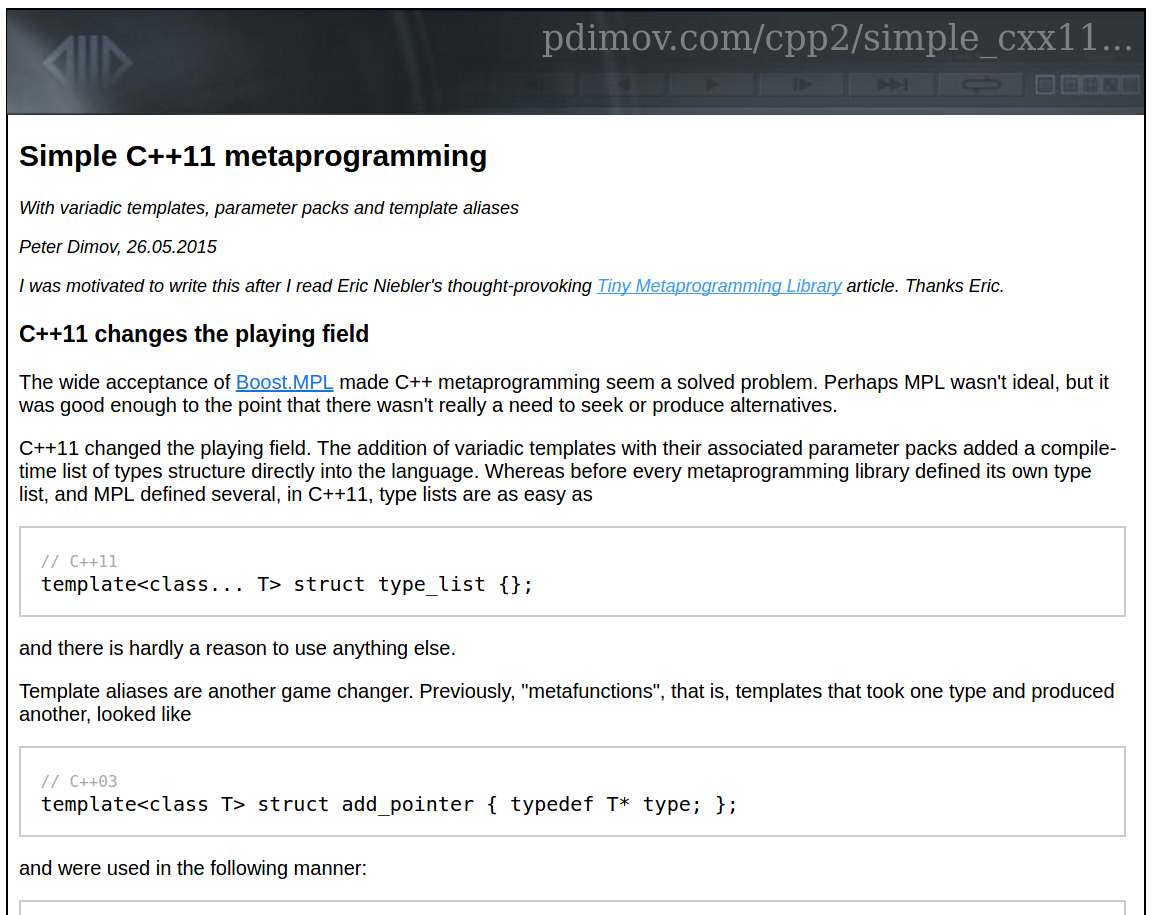
\includegraphics[width=0.99\textwidth]{pdimov}
      \end{figure}
    \end{column}%
  \end{columns}
\end{frame}


\begin{frame}[plain]
      \begin{figure}[H]
        \centering
        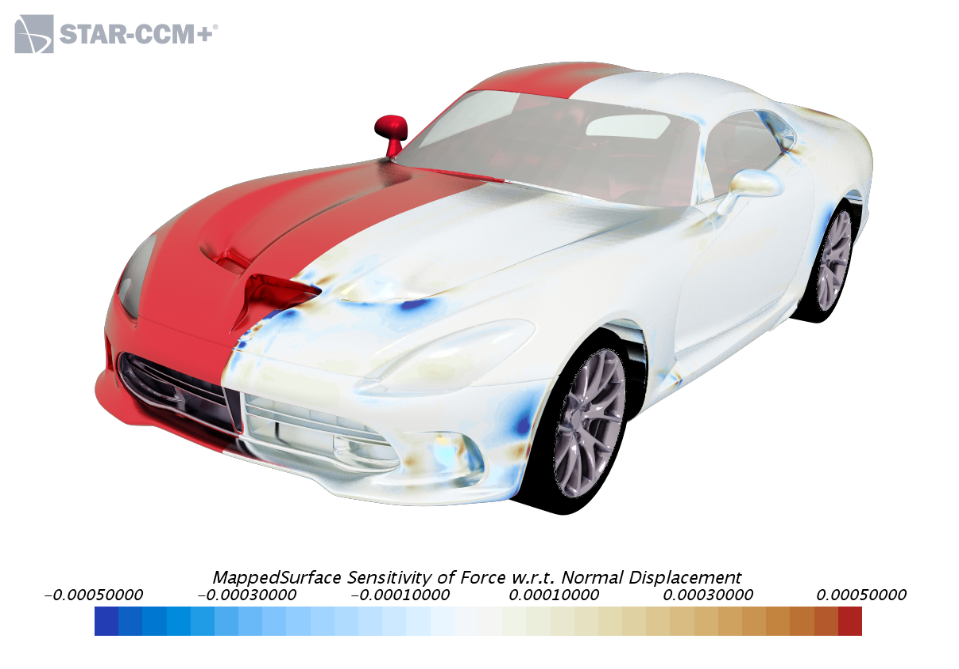
\includegraphics[width=0.99\textwidth]{jag_surf_opt}
        \caption{Compressible N-S adjoint: automatic at loop iteration level}
      \end{figure}
\end{frame}


%%
\section{Differentiate a function \protect\textit{losslessly}}
%%

\begin{frame}[fragile]{Parity preserving transform}
  \begin{columns}[T] % align columns
    \begin{column}{0.44\textwidth}
      {\color{gray}{write something like this \dots}}
      \begin{lstlisting}
fn(A const &a, B const &b,
   R &r)
{
  auto c0 = 7;
  auto c1 = 9;

  auto t0 = a * b;   // 1
  auto t1 = c0 + t0; // 2
  auto t2 = c1 + t0; // 3

  r  = t1 / t2;      // 4
}
  \end{lstlisting}
    \end{column}%
    \hfill%
    \begin{column}{0.56\textwidth}
      {\color{gray}{to implement something like this}}
        \begin{lstlisting}
fn(A const &a, B const &b,
   R &r)
{
  auto c0 = 7;
  auto c1 = 9;

  auto t0 = a * b;   // 1
  auto t1 = c0 + t0; // 2
  auto t2 = c1 + t0; // 3

  // somehow add this...
  t1.d += (1/t2)    * r.d; // 4'
  t2.d -= (t1/t2^2) * r.d; // 4'
  t0.d += t2.d;            // 3'
  t0.d += t1.d;            // 2'
  a.d  += b * t0.d;        // 1'
  b.d  += a * t0.d;        // 1'
}
  \end{lstlisting}
    \end{column}%
  \end{columns}
\end{frame}


\begin{frame}[fragile]{Observations}
  \begin{enumerate}
  \item Given a pure-functional algorithm, differentiate it \vspace{5mm}
  \item Implement the transpose of the chain of derivatives (the adjoint) \vspace{5mm}
  \item The required `extra' code is in the reversed sequence of the original and the data flow is reversed \vspace{5mm}
  \item Eager and lazy evaluation: ctor-dtor pairs? \vspace{5mm}
  \end{enumerate}
\end{frame}

%%
\section{Two hurdles}
%%

\begin{frame}[fragile]{1. Dealing with duplicate nodes}
Eager evaluation and capture by reference?
  \begin{columns}[T] % align columns
    \begin{column}{0.5\textwidth}
        \begin{lstlisting}
fn(A const &a, B const &b,
   R &r)
{
  auto c0 = 7;
  auto c1 = 9;

  auto @\aftergroup\bluecolor@t0@\aftergroup\blackcolor@ = a * b;
  auto t1 = c0 + @\aftergroup\bluecolor@t0@\aftergroup\blackcolor@;
  auto t2 = c1 + @\aftergroup\bluecolor@t0@\aftergroup\blackcolor@;

  r  = t1 / t2;
}
  \end{lstlisting}
    \end{column}%
    \hfill%
    \begin{column}{0.5\textwidth}
\begin{figure}[H]
 \centering
 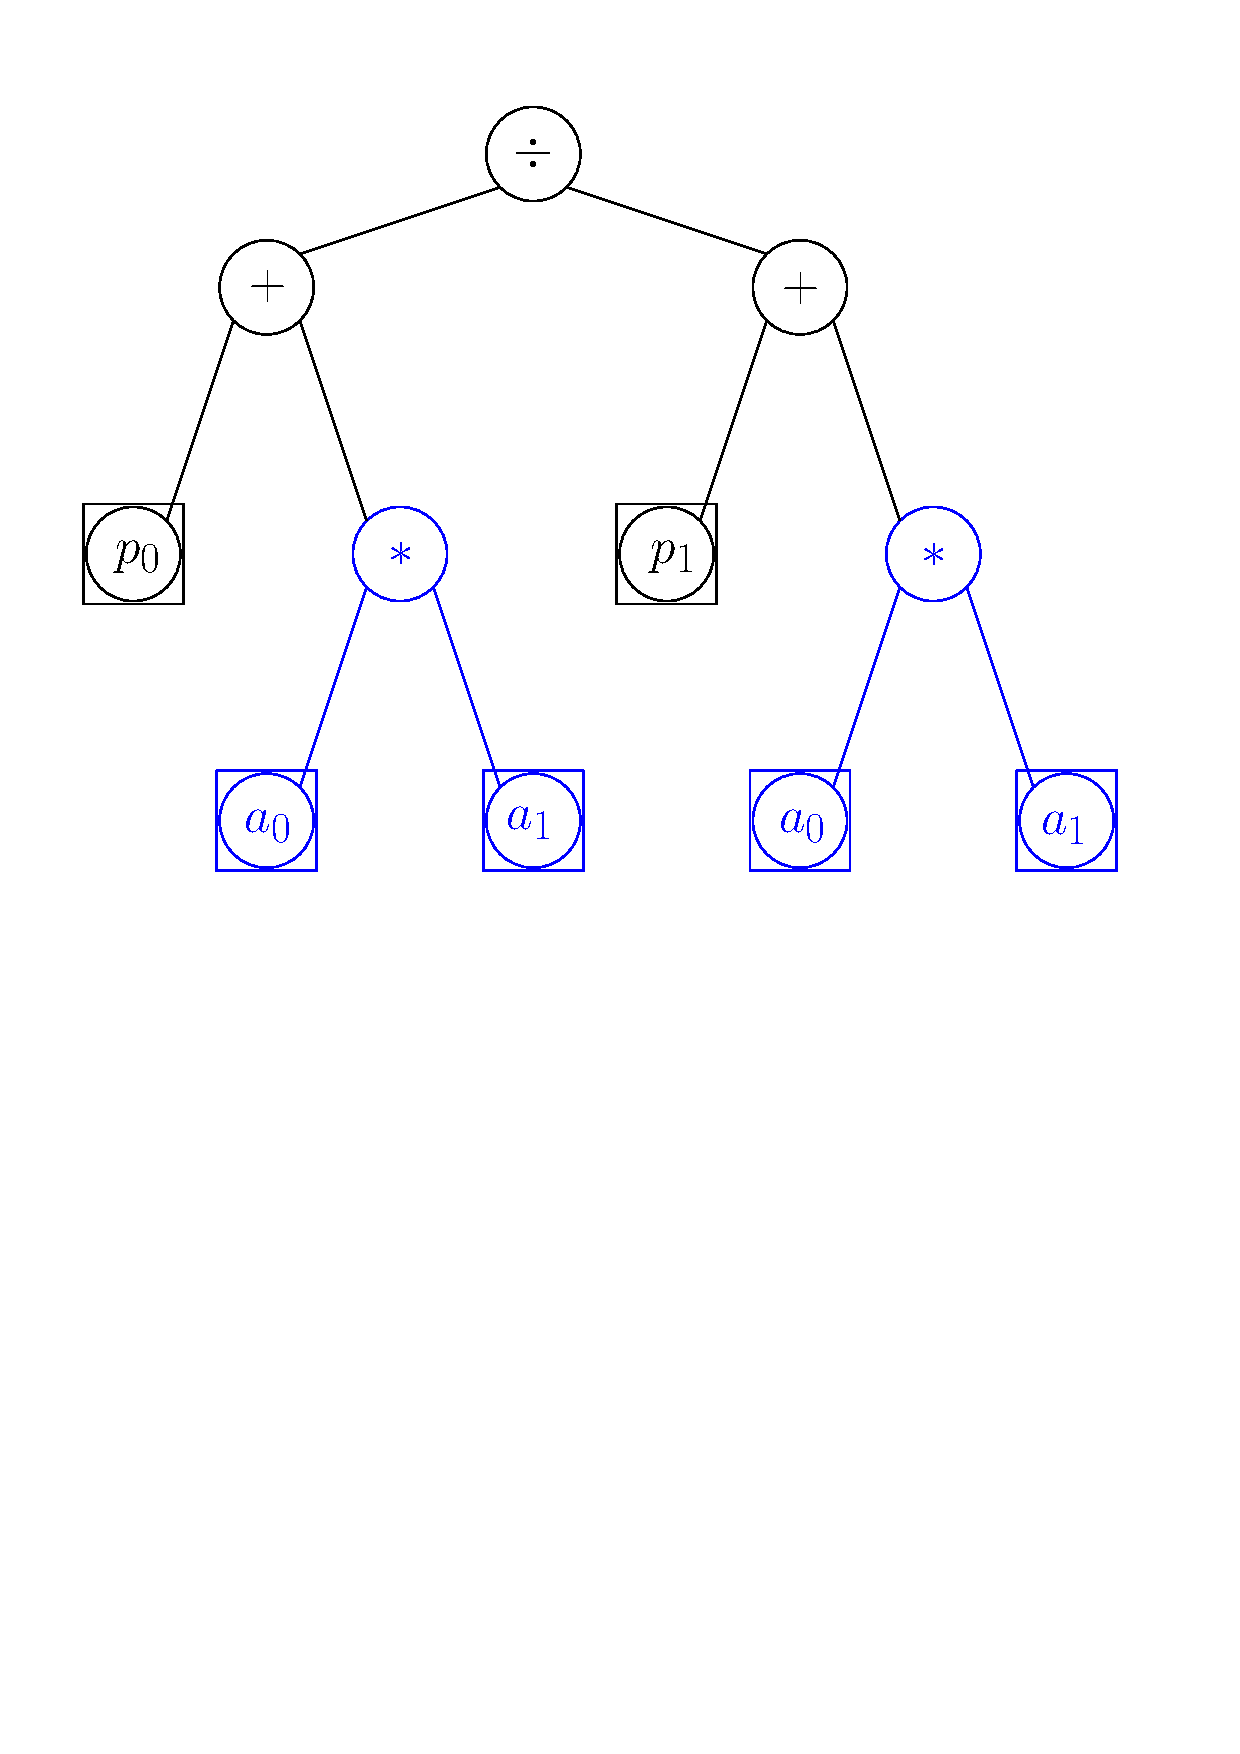
\includegraphics[width=0.99\textwidth]{fig_exprtree_dup}
\end{figure}
    \end{column}%
  \end{columns}
\end{frame}


\begin{frame}[fragile]{2. Dealing with nested scoping}
The \emph{complete} tree, including {\color{red}\texttt{cm}}, is needed for the transform

      \begin{lstlisting}
@\aftergroup\bluecolor@mul_dbl@\aftergroup\blackcolor@(A const &a, B const &b)
{
  auto @\aftergroup\redcolor@cm@\aftergroup\blackcolor@ = 2; // locally scoped
  return @\aftergroup\redcolor@cm@\aftergroup\blackcolor@ * a * b;
}

fn(A const &a, B const &b, R &r)
{
  auto c0 = 7;
  auto c1 = 9;

  auto t0 = @\aftergroup\bluecolor@mul_dbl(a, b)@\aftergroup\blackcolor@;
  auto t1 = c0 + t0;
  auto t2 = c1 + t0;

  r  = t1 / t2;
}
  \end{lstlisting}
\end{frame}


\begin{frame}[fragile]{2. Dealing with nested scoping}
The \emph{complete} tree, including {\color{red}\texttt{cm}}, is needed for the transform
  \begin{columns}[T] % align columns
    \begin{column}{0.44\textwidth}
      \begin{lstlisting}
fn(A const &a, B const &b,
   R &r)
{
  auto c0 = 7;
  auto c1 = 9;
  auto @\aftergroup\redcolor@cm@\aftergroup\blackcolor@ = 2;
  auto t0 = @\aftergroup\redcolor@cm@\aftergroup\blackcolor@ * a * b;
  auto t1 = c0 + t0;
  auto t2 = c1 + t0;

  r  = t1 / t2;
}
  \end{lstlisting}
    \end{column}%
    \hfill%
    \begin{column}{0.56\textwidth}
        \begin{lstlisting}
fn(A const &a, B const &b,
   R &r)
{
  auto c0 = 7;
  auto c1 = 9;
  auto @\aftergroup\redcolor@cm@\aftergroup\blackcolor@ = 2;
  auto t0 = @\aftergroup\redcolor@cm@\aftergroup\blackcolor@ * a * b;
  auto t1 = c0 + t0;
  auto t2 = c1 + t0;

  // the transform...
  t1.d += (1/t2)    * r.d;
  t2.d -= (t1/t2^2) * r.d;
  t0.d += t2.d;
  t0.d += t1.d;
  a.d  += @\aftergroup\redcolor@cm@\aftergroup\blackcolor@ * b * t0.d;
  b.d  += @\aftergroup\redcolor@cm@\aftergroup\blackcolor@ * a * t0.d;
}
  \end{lstlisting}
    \end{column}%
  \end{columns}
\end{frame}


\begin{frame}[fragile]{State of affairs}
  \begin{enumerate}
  \item Eager evaluation avoids duplicate branch evaluation - but lazy evaluation will also be needed \vspace{5mm}
  \item `Capture by reference' to keep the tree small - but cannot work with nested scoping \vspace{5mm}
  \item `Capture by value' is too inefficient - the tree will get very large very quickly \vspace{5mm}
  \item A monolithic tree, supporting eager and lazy evaluation, of minimal size, and impartial to scoping is required \vspace{5mm}
  \end{enumerate}
\end{frame}


%%
\section{Expression tree to type list}
%%

\begin{frame}[fragile]{Two kinds of data}
\begin{lstlisting}
auto fn(A const &@\aftergroup\redcolor@a@\aftergroup\blackcolor@, B const &@\aftergroup\redcolor@b@\aftergroup\blackcolor@)
{
  auto @\aftergroup\bluecolor@c0@\aftergroup\blackcolor@ = @\aftergroup\greencolor@UQ(@\aftergroup\blackcolor@7@\aftergroup\greencolor@)@\aftergroup\blackcolor@;
  auto @\aftergroup\bluecolor@c1@\aftergroup\blackcolor@ = @\aftergroup\greencolor@UQ(@\aftergroup\blackcolor@9@\aftergroup\greencolor@)@\aftergroup\blackcolor@;

  auto t0 = @\aftergroup\redcolor@a@\aftergroup\blackcolor@ * @\aftergroup\redcolor@b@\aftergroup\blackcolor@;
  auto t1 = @\aftergroup\bluecolor@c0@\aftergroup\blackcolor@ + t0;
  auto t2 = @\aftergroup\bluecolor@c1@\aftergroup\blackcolor@ + t0;
  return t1 / t2;
}
\end{lstlisting}
\end{frame}


\begin{frame}[fragile]{Two kinds of data}
  \begin{columns}[T] % align columns
    %% \begin{column}{0.3\textwidth}
    %% \end{column}%
    %% \hfill%
    \begin{column}{0.75\textwidth}
      \begin{figure}[H]
        \centering
        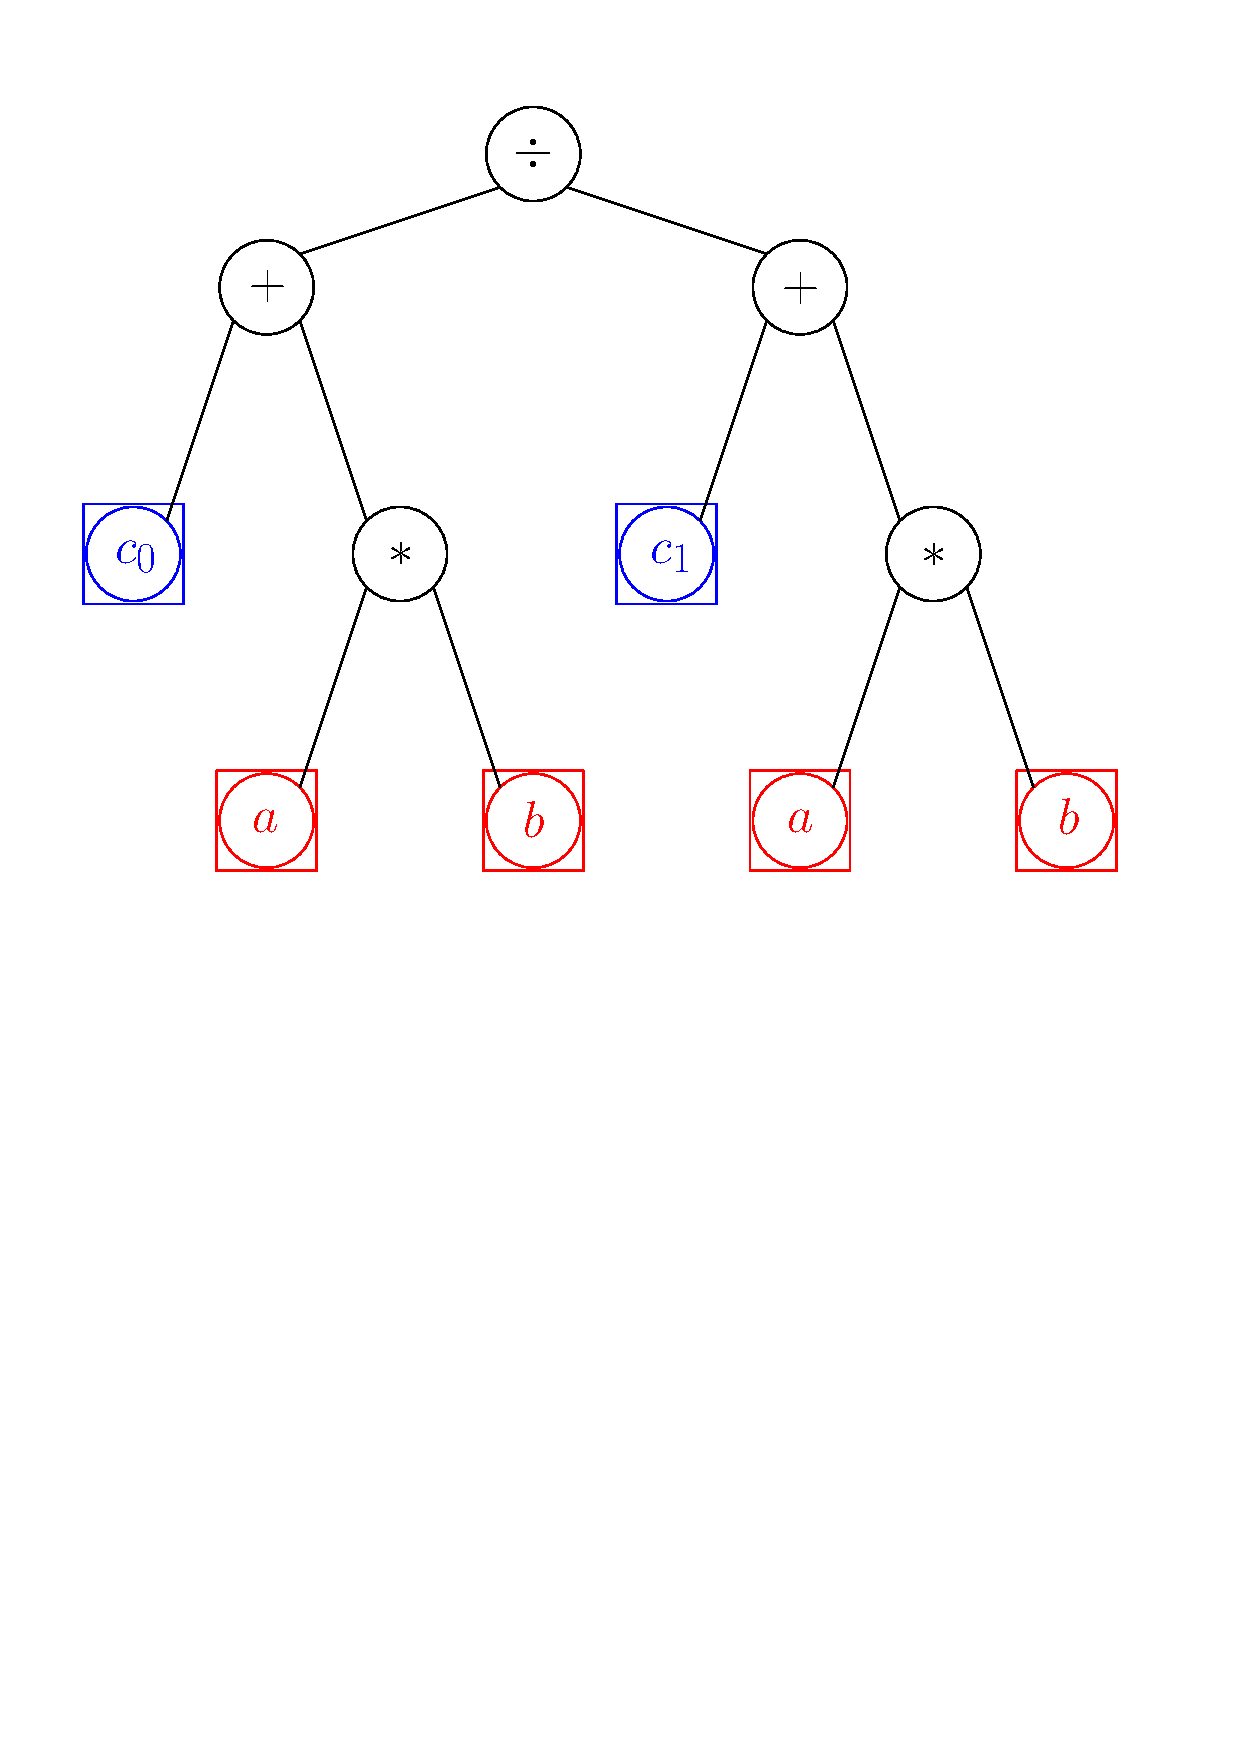
\includegraphics[width=0.99\textwidth]{fig_exprtree_cb_rb}
      \end{figure}
    \end{column}%
  \end{columns}
\end{frame}


\begin{frame}[fragile]{\texttt{UQ}}
\begin{lstlisting}
template<std::size_t ID, typename T>
struct Unique
{
  T value;
};
\end{lstlisting}

~

\begin{lstlisting}
// UQ
@\aftergroup\bluecolor@#define UQ(v) Unique<__COUNTER__, decltype(v)>{v}@\aftergroup\blackcolor@
\end{lstlisting}
\end{frame}


\begin{frame}[fragile]{Tree type to list of types}
Generate tree with operator overloading
\begin{lstlisting}
  Binary<Div,
    Binary<Add, @\aftergroup\bluecolor@C0@\aftergroup\blackcolor@,
      Binary<Mul, @\aftergroup\redcolor@A@\aftergroup\blackcolor@, @\aftergroup\redcolor@B@\aftergroup\blackcolor@> >
    Binary<Add, @\aftergroup\bluecolor@C1@\aftergroup\blackcolor@,
      Binary<Mul, @\aftergroup\redcolor@A@\aftergroup\blackcolor@, @\aftergroup\redcolor@B@\aftergroup\blackcolor@> > >
\end{lstlisting}

~

Group hierarchically and prune duplicates (at each binary node),\newline
then flatten (at the root node)
\begin{lstlisting}
 {@\aftergroup\redcolor@A@\aftergroup\blackcolor@,
  @\aftergroup\redcolor@B@\aftergroup\blackcolor@,
  Binary<Mul, @\aftergroup\redcolor@A@\aftergroup\blackcolor@, @\aftergroup\redcolor@B@\aftergroup\blackcolor@>,
  Binary<Add, @\aftergroup\bluecolor@C0@\aftergroup\blackcolor@, [...]>,
  Binary<Add, @\aftergroup\bluecolor@C1@\aftergroup\blackcolor@, [...]>,
  Binary<Div, [...], [...]>}
\end{lstlisting}
\end{frame}


\begin{frame}[fragile]{Mapping nodes to data}
Map {\color{blue}\texttt{C0}} and {\color{blue}\texttt{C1}} to values
\begin{lstlisting}
  L = {@\aftergroup\redcolor@A@\aftergroup\blackcolor@,                                //  0
       @\aftergroup\redcolor@B@\aftergroup\blackcolor@,                                //  1
       Binary<Mul, @\aftergroup\redcolor@A@\aftergroup\blackcolor@, @\aftergroup\redcolor@B@\aftergroup\blackcolor@>,                //  2
       Binary<Add, @\aftergroup\bluecolor@C0@\aftergroup\blackcolor@, [...]>,           //  3  <--
       Binary<Add, @\aftergroup\bluecolor@C1@\aftergroup\blackcolor@, [...]>,           //  4  <--
       Binary<Div, [...], [...]>}        //  5
\end{lstlisting}
%%
\begin{lstlisting}
  tuple<float, float> @\aftergroup\bluecolor@vars@\aftergroup\blackcolor@ = {7.0, 9.0};
\end{lstlisting}

~

Indices of constants in `\texttt{L}'
\begin{lstlisting}
  @\aftergroup\bluecolor@IC@\aftergroup\blackcolor@ = {3, 4}
\end{lstlisting}

~

Map elements in `\texttt{L}' to storage offsets \emph{(2 = null marker)}
\begin{lstlisting}
  @\aftergroup\bluecolor@DC@\aftergroup\blackcolor@ = {2, 2, 2, @\aftergroup\bluecolor@0@\aftergroup\blackcolor@, @\aftergroup\bluecolor@1@\aftergroup\blackcolor@, 2}
\end{lstlisting}
\end{frame}


\begin{frame}[fragile]{\texttt{dual}}
\begin{lstlisting}
// input                                output
//-------                              --------
@\aftergroup\bluecolor@DC_SIZE@\aftergroup\blackcolor@ = 6     \
                 --- @\aftergroup\blackcolor@dual@\aftergroup\blackcolor@ --->    @\aftergroup\bluecolor@DC@\aftergroup\blackcolor@ = {2, 2, 2, 0, 1, 2}
@\aftergroup\bluecolor@IC@\aftergroup\blackcolor@ = {3, 4}     /                       @\aftergroup\graycolor@0  1  2  3  4  5@\aftergroup\blackcolor@
\end{lstlisting}

~

\vspace{5mm}
\footnotesize{\texttt{github.com/DominicJones/snippets/blob/master/Cxx/mp\_functions.cpp}}
\end{frame}


\begin{frame}[fragile]{Mapping nodes to data}
Map {\color{red}\texttt{A}} and {\color{red}\texttt{A}} to addresses
\begin{lstlisting}
  L = {@\aftergroup\redcolor@A@\aftergroup\blackcolor@,                                //  0  <--
       @\aftergroup\redcolor@B@\aftergroup\blackcolor@,                                //  1  <--
       Binary<Mul, @\aftergroup\redcolor@A@\aftergroup\blackcolor@, @\aftergroup\redcolor@B@\aftergroup\blackcolor@>,                //  2
       Binary<Add, @\aftergroup\bluecolor@C0@\aftergroup\blackcolor@, [...]>,           //  3
       Binary<Add, @\aftergroup\bluecolor@C1@\aftergroup\blackcolor@, [...]>,           //  4
       Binary<Div, [...], [...]>}        //  5
\end{lstlisting}
%%
\begin{lstlisting}
  tuple<float*, float*> @\aftergroup\redcolor@args@\aftergroup\blackcolor@ = {&@\aftergroup\redcolor@a@\aftergroup\blackcolor@, &@\aftergroup\redcolor@b@\aftergroup\blackcolor@};
\end{lstlisting}


~

Map offsets of left child nodes \emph{(6 = null marker)}
\begin{lstlisting}
  IL_L = {6, 6, @\aftergroup\redcolor@0@\aftergroup\blackcolor@, 6, 6, 3}
\end{lstlisting}

~

Map offsets of right child nodes
\begin{lstlisting}
  IL_R = {6, 6, @\aftergroup\redcolor@1@\aftergroup\blackcolor@, 2, 2, 4}
\end{lstlisting}
\end{frame}


\begin{frame}[fragile]{Evaluate operator list}
%%
\begin{lstlisting}
  tuple<float, float> @\aftergroup\bluecolor@vars@\aftergroup\blackcolor@   = {7.0, 9.0};
\end{lstlisting}
%%
\begin{lstlisting}
  tuple<float*, float*> @\aftergroup\redcolor@args@\aftergroup\blackcolor@ = {&@\aftergroup\redcolor@a@\aftergroup\blackcolor@, &@\aftergroup\redcolor@b@\aftergroup\blackcolor@};
\end{lstlisting}

~

\begin{lstlisting}
  @\aftergroup\bluecolor@DC@\aftergroup\blackcolor@   = {2, 2, 2, @\aftergroup\bluecolor@0@\aftergroup\blackcolor@, @\aftergroup\bluecolor@1@\aftergroup\blackcolor@, 2}
\end{lstlisting}
%%
\begin{lstlisting}
  IL_L = {6, 6, @\aftergroup\redcolor@0@\aftergroup\blackcolor@, 6, 6, 3}
\end{lstlisting}
%%
\begin{lstlisting}
  IL_R = {6, 6, @\aftergroup\redcolor@1@\aftergroup\blackcolor@, 2, 2, 4}
\end{lstlisting}

~

Iterate list to compute primal and adjoint
\begin{lstlisting}
  L = {@\aftergroup\redcolor@A@\aftergroup\blackcolor@,                                //  0
       @\aftergroup\redcolor@B@\aftergroup\blackcolor@,                                //  1
       Binary<Mul, @\aftergroup\redcolor@A@\aftergroup\blackcolor@, @\aftergroup\redcolor@B@\aftergroup\blackcolor@>,                //  2
       Binary<Add, @\aftergroup\bluecolor@C0@\aftergroup\blackcolor@, [...]>,           //  3
       Binary<Add, @\aftergroup\bluecolor@C1@\aftergroup\blackcolor@, [...]>,           //  4
       Binary<Div, [...], [...]>}        //  5
\end{lstlisting}
\end{frame}


\begin{frame}[fragile]{Results}
\textbf{Case 1}: nodes: 82, depth: 37, inputs: 2, constants: 12
\begin{table}
\begin{tabular}{l | c | c | c | c }
Version & compilation & original & auto diff & manual diff \\
\hline \hline
\texttt{alt::tuple} & 2.2s & 1x & 1.25x & 1.48x \\
\texttt{std::tuple} & 4.5s & 1x & 1.25x & 1.48x \\
\end{tabular}
\end{table}
\vspace{10mm}
\textbf{Case 2}: nodes: 331, depth: 25, inputs: 5, constants: 103
\begin{table}
\begin{tabular}{l | c | c | c | c }
Version & compilation & original & auto diff & manual diff \\
\hline \hline
\texttt{alt::tuple} & 59s & 1x & 5.7x & 1.9x \\
\texttt{std::tuple} & 27m & 1x & 4.7x & 1.9x \\
\end{tabular}
\end{table}
\end{frame}


\begin{frame}[fragile]{Conclusion}
  \begin{enumerate}
  \item Manipulation the tree is obtained at immense effort \vspace{3mm}
  \item Works in the range of exceptionally well (better than hand coded) to acceptably well (better than alternatives) \vspace{5mm}
  \item Compile-time features of the language are too limited to use this approach neatly (cf. preprocessor macros) \vspace{3mm}
  \item Inlining gives up too readily; \verb$__attribute__((always_inline))$ used ubiquitously \vspace{3mm}
  \item Only supports having one result \vspace{3mm}
  \item Not obvious what is going on with \verb$std::tuple$ \vspace{3mm}
  \end{enumerate}
\end{frame}


%%
\section{\protect\textit{Float template parameter}}
%%

\begin{frame}[fragile]{Distinguishing different constants}
  \begin{columns}[T] % align columns
    %% \begin{column}{0.3\textwidth}
    %% \end{column}%
    %% \hfill%
    \begin{column}{0.75\textwidth}
      \begin{figure}[H]
        \centering
        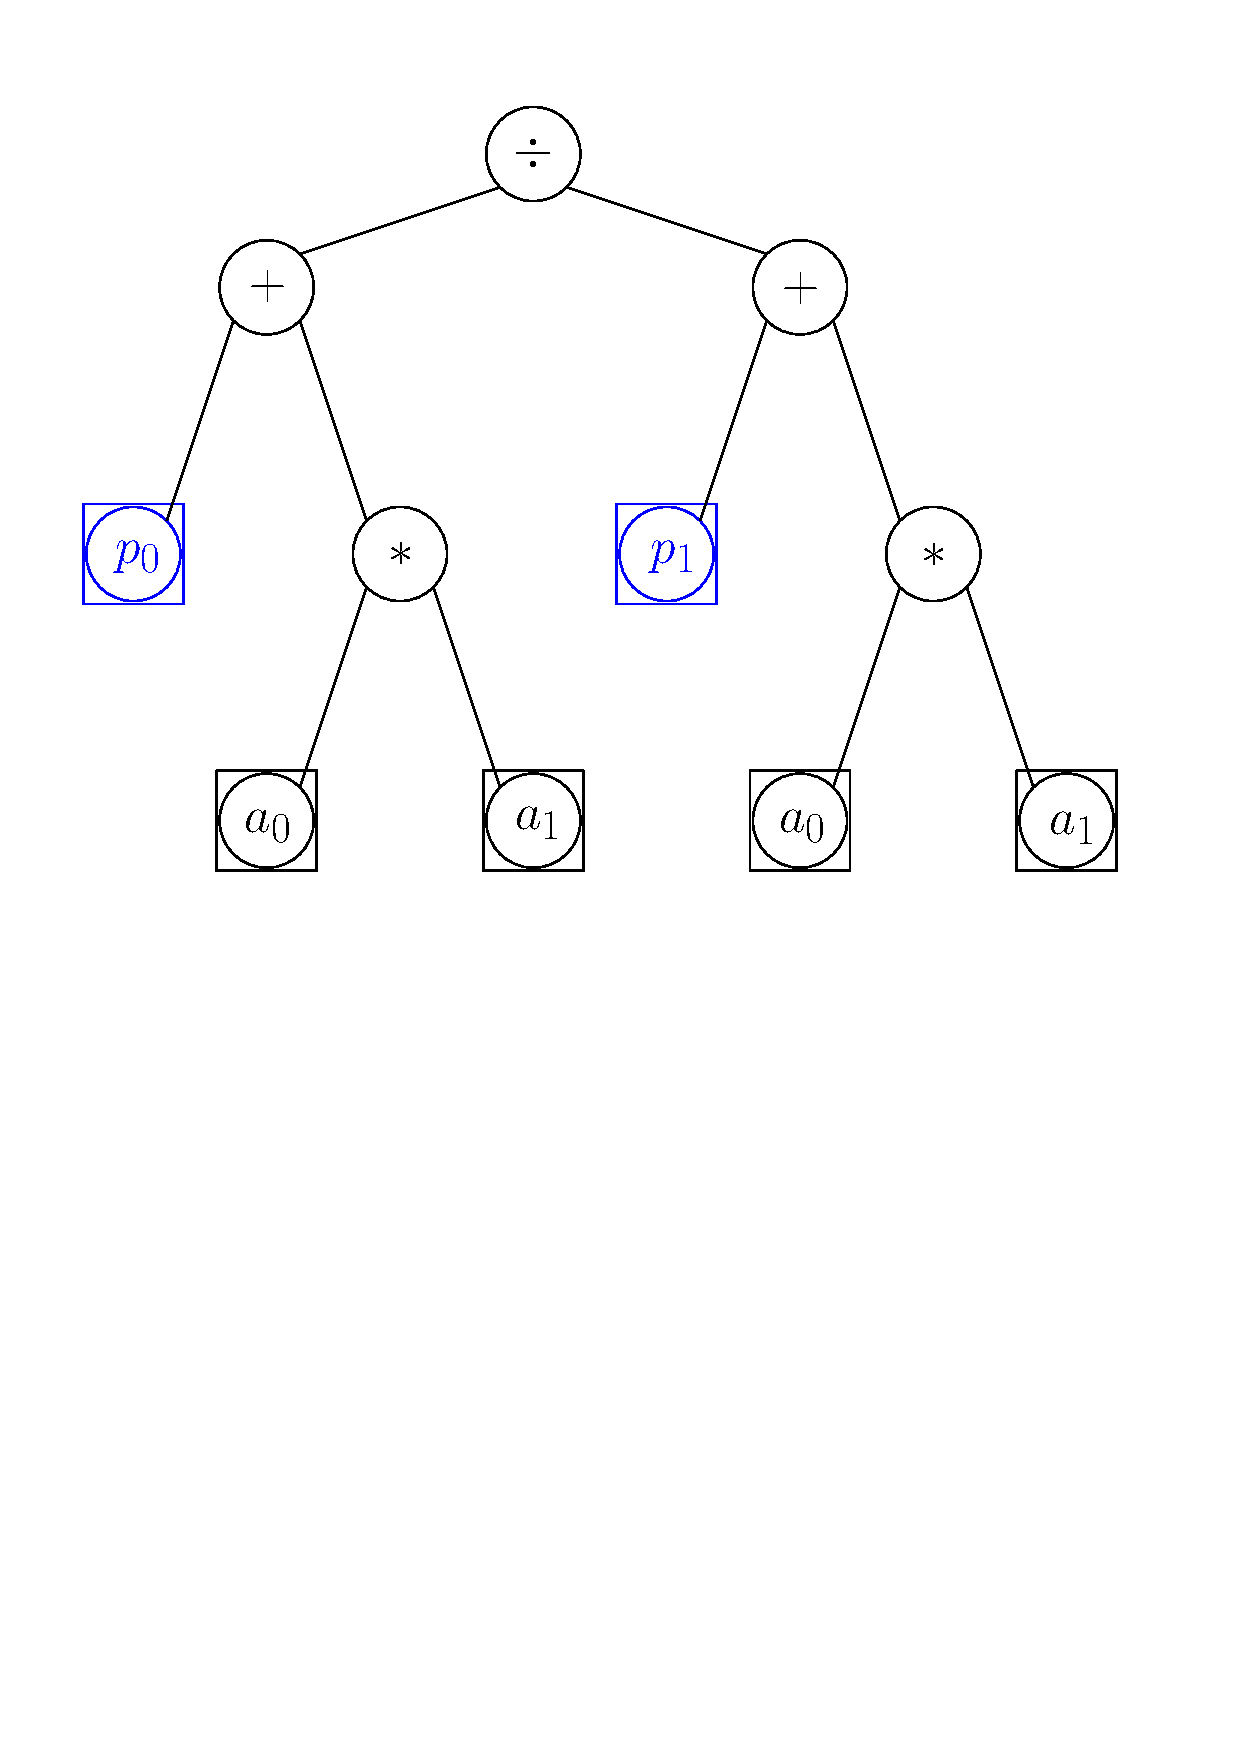
\includegraphics[width=0.99\textwidth]{fig_exprtree_cb}
      \end{figure}
    \end{column}%
  \end{columns}
\end{frame}


\begin{frame}[fragile]{\dangersign \emph{Values as types} \dangersign}
\begin{lstlisting}
// C++ does not permit `auto' to resolve as `float'
template<auto V>
struct @\aftergroup\redcolor@_float@\aftergroup\blackcolor@
{
  constexpr operator auto() const { return V; }
};
\end{lstlisting}

~

\begin{lstlisting}
// type distinguished by value
auto constexpr @\aftergroup\bluecolor@c0@\aftergroup\blackcolor@ = -4.2@\aftergroup\redcolor@_f@\aftergroup\blackcolor@;
static_assert(@\aftergroup\bluecolor@c0@\aftergroup\blackcolor@ == @\aftergroup\redcolor@_float@\aftergroup\blackcolor@<-4.2>{});
\end{lstlisting}
\end{frame}


\begin{frame}[fragile]{Values as types in D}
\begin{lstlisting}
// exactly what is wanted
struct _float(@\aftergroup\bluecolor@float@\aftergroup\blackcolor@ v)
{
  static immutable auto value = v;
}
\end{lstlisting}
\end{frame}


\begin{frame}[fragile]{``\texttt{\_float}'' \emph{workaround}}
\begin{lstlisting}
// exponent ignored...
template<auto H, auto L, auto E>
struct _float
{
  auto constexpr static value =
    (H + @\aftergroup\bluecolor@float@\aftergroup\blackcolor@(L) / multiplier<10, E, 1>::value);

  constexpr operator auto() const { return value; }
};
\end{lstlisting}

~

\begin{lstlisting}
// and for operator+
template<auto H, auto L, auto E>
auto constexpr operator-(_float<H, L, E>)
{
  return _float<(-H), (-L), E>{};
}
\end{lstlisting}
\end{frame}


\begin{frame}[fragile]{\ldots made palatable}
\begin{lstlisting}
// makes life easier
template<char...> struct mp_chars {};
\end{lstlisting}

~

\begin{lstlisting}
// user-defined literal
template<char... Cs>
auto constexpr operator""@\aftergroup\bluecolor@_f@\aftergroup\blackcolor@()
{
  return @\aftergroup\redcolor@make_float_t@\aftergroup\blackcolor@<0, 0, 0, 0,
                      sizeof...(Cs), mp_chars<Cs...> >{};
}
\end{lstlisting}

~

\begin{lstlisting}
// seamless conversion to literals
auto constexpr c0 = -4.2@\aftergroup\bluecolor@_f@\aftergroup\blackcolor@;
float t0 = 2 * c0;
\end{lstlisting}
\end{frame}


%% \begin{frame}[fragile]{Parsing}
%% \begin{lstlisting}

%%   123.45@\aftergroup\bluecolor@_f@\aftergroup\blackcolor@

%%   // represented as
%%   mp_chars<'1', '2', '3', '.', '4', '5'>

%%   H = '1', '2', '3'  // high chars
%%   L = '4', '5'       // low chars
%%   E = 4              // decimal offset
%%   N = 6              // length

%% \end{lstlisting}
%% \end{frame}


%% \begin{frame}[fragile]{Terminal}
%% \begin{lstlisting}
%% // still have a terminal function
%% template<auto H, auto L, auto E,
%%          auto I, auto N,
%%          template<char...> class CL>
%% auto constexpr make_float_fn(CL<> cl)
%% {
%%   return _float<H, L, (N - E)>{};
%% }
%% \end{lstlisting}
%% \end{frame}


%% \begin{frame}[fragile]{Decimal offset and digits}
%% \begin{lstlisting}
%% // return type deduced...
%% template<auto H, auto L, auto E,
%%          auto I, auto N,
%%          template<char,char...> class CL, char C, char... Cs>
%% @\aftergroup\bluecolor@auto@\aftergroup\blackcolor@ constexpr make_float_fn(CL<C, Cs...> cl)
%% {
%%   @\aftergroup\redcolor@if constexpr@\aftergroup\blackcolor@ (C == '.')
%%   {
%%     auto constexpr _E = I + 1;
%%     @\aftergroup\bluecolor@return@\aftergroup\blackcolor@ make_float_fn<H, L, _E, (I+1), N>(CL<Cs...>{});
%%   }
%%   else
%%   {
%%     auto constexpr _D = (C >= '0' && C <= '9');
%%     auto constexpr _H = (_D && E == 0)? 10*H+(C-'0'): H;
%%     auto constexpr _L = (_D && E  > 0)? 10*L+(C-'0'): L;
%%     @\aftergroup\bluecolor@return@\aftergroup\blackcolor@ make_float_fn<_H, L, E, (I+1), N>(CL<Cs...>{});
%%   }
%% }
%% \end{lstlisting}
%% \end{frame}


%%
\section{\protect\textit{Reflect variable location}}
%%


\begin{frame}[fragile]{The trusty preprocessor}
\begin{lstlisting}
auto fn(A const &@\aftergroup\redcolor@a@\aftergroup\blackcolor@, B const &@\aftergroup\redcolor@b@\aftergroup\blackcolor@)
{
  auto @\aftergroup\bluecolor@c0@\aftergroup\blackcolor@ = @\aftergroup\greencolor@UQ(@\aftergroup\blackcolor@7@\aftergroup\greencolor@)@\aftergroup\blackcolor@; // auto = Unique<724, float>{7}
  auto @\aftergroup\bluecolor@c1@\aftergroup\blackcolor@ = @\aftergroup\greencolor@UQ(@\aftergroup\blackcolor@9@\aftergroup\greencolor@)@\aftergroup\blackcolor@; // auto = Unique<725, float>{9}

  auto t0 = @\aftergroup\redcolor@a@\aftergroup\blackcolor@ * @\aftergroup\redcolor@b@\aftergroup\blackcolor@;
  auto t1 = @\aftergroup\bluecolor@c0@\aftergroup\blackcolor@ + t0;
  auto t2 = @\aftergroup\bluecolor@c1@\aftergroup\blackcolor@ + t0;
  return t1 / t2;
}
\end{lstlisting}
\end{frame}


\begin{frame}[fragile]{A fundamental problem}
Write a \texttt{transform} function to yield:\vspace{10mm}
\begin{lstlisting}
  auto @\aftergroup\bluecolor@c0@\aftergroup\blackcolor@ = 7;
  auto @\aftergroup\bluecolor@c1@\aftergroup\blackcolor@ = 9;

  transform(@\aftergroup\bluecolor@c0 + c0@\aftergroup\blackcolor@)  -->   @\aftergroup\redcolor@2 * c0@\aftergroup\blackcolor@
  transform(@\aftergroup\bluecolor@c1 + c0@\aftergroup\blackcolor@)  -->  @\aftergroup\bluecolor@c1 + c0@\aftergroup\blackcolor@
\end{lstlisting}
\vspace{10mm}
\emph{Impossible!}
\ldots despite it appearing so trivial
\end{frame}


\begin{frame}[fragile]{Three kinds of reflection?}
  \begin{lstlisting}

@\aftergroup\graycolor@ 123456789 123456789 123456789
          10        20        30
1
2  // main.cpp
3
4@\aftergroup\blackcolor@  decltype(@\aftergroup\bluecolor@x@\aftergroup\blackcolor@)*   y   =   &@\aftergroup\bluecolor@x@\aftergroup\blackcolor@;@\aftergroup\graycolor@
5

@\aftergroup\greencolor@     reflect             reflect
     type                address@\aftergroup\graycolor@
  \end{lstlisting}
 \vspace{10mm}
Reflect \emph{location} of {\color{blue}\texttt{x}}, at {\color{red}\texttt{[7, 4, main.cpp]}}?
\end{frame}


\begin{frame}[fragile]{Reflect location in D}
\begin{lstlisting}
struct Terminal(T, string file = @\aftergroup\bluecolor@__FILE__@\aftergroup\blackcolor@,
                   size_t line = @\aftergroup\bluecolor@__LINE__@\aftergroup\blackcolor@)
{
  T value;

  ...
}
\end{lstlisting}

~

\begin{lstlisting}
Terminal!double @\aftergroup\bluecolor@c0@\aftergroup\blackcolor@ = 7; // Terminal<double, "main.d", 724>
Terminal!double @\aftergroup\bluecolor@c1@\aftergroup\blackcolor@ = 9; // Terminal<double, "main.d", 725>
\end{lstlisting}

\vspace{10mm}
{One definition per line could be run-time checked with a debug build which requires all \texttt{Terminal}s be singletons.}
\end{frame}


%%
\begin{frame}[plain]
  \titlepage
\end{frame}
%%
\end{document}
